\chapter{Analysis}

\section{Background Research}
\subsection{Graphics}
For my project, I am thinking of using a third party graphics library to make it simple to create a sphere, without having to go low level. \\
I could write the graphics from scratch using \verb|WebGL|, however I feel like this is quite low level, and requires a lot of unnecessary time waste when I could just import a bare bones library. \\
A library that interests me is \verb|THREE.js|\footnote{https://threejs.org}, it is specifically a graphics library, so no time spent having to work with object physics. It also has strong documentation, a wide variety of examples, and a lot of real world uses. It's free, and it's also built to be a single file, which means it'll be easy to import into my project.
An alternative is \verb|babylon.js|\footnote{https://www.babylonjs.com}, it comes with many tools allowing for easy production, as well as a graphical tool that allows you to chain systems and create materials and textures without a single line of code. The problem I have with this is that I think it's too much, I don't think these tools will save me much time, and are hard to move to other computers. \\

I will probably create my project using \verb|THREE.js|.

\newpage
\subsection{APIs}
For the retrieval of country information there are two ways of doing it, calling an API and retrieving the information that way, or storing all the information on a local database and retrieving it that way. \\
The reason I am choosing the former is because I think requesting information from an API is a simpler option. It does have its drawbacks, however. I have plotted some pros and cons regarding this:
\begin{center}
\begin{tabular}{|p{3cm}|p{3cm}|p{3cm}|p{3cm}|}
\hline
\multicolumn{2}{|c|}{API Requesting} &
\multicolumn{2}{|c|}{Local Database} \\
\hline
Advantages & Disadvantages & Advantages & Disadvantages \\
\hline
Easy & Potentially slow & Fast & Requires hosting \\
Simple & Request limitations & No request limits & Complex \\
No storage space\linebreak needed & Not tailored & Customizable & Large file size \\
\hline
\end{tabular}
\end{center}
Since I am not seeking speed, and I am theoretically requesting with no limits, I think that I should use API Requesting to keep my project back-end simple. \\
I now need to choose a good API, the attributes I am looking for when searching for an API are:
\begin{itemize}
\itemsep0em
\item It must be free to use, or be publicly hosted.
\item It must be relevant to this project.
\item It should require no login.
\item It should contain information in regards to a specific country. (in other words, be able to accept \verb|POST| requests)
\item It could contain extra relevant information.
\end{itemize}
The first public API I came across was 'worldpop.org'\footnote{https://www.worldpop.org}, it contains numerous interfaces for demographics, and has real world use for demographic research. It contains data like, births, urban changes, population history, etc...
What I concluded from looking at worldpop was the fact that it is too specific, for example, to find the population of a country, it requires a certain radius of resolution - essentially, I cannot simply search for a country and retrieve its population. \\
\newpage
The second public API I came across was 'countriesnow.space'\footnote{https://countriesnow.space}, I like it for its simplicity. It's a lightweight API with quite descriptive yet simple documentation and allows for filtering using SQL-like queries. It contains data such as population data for a country and city, flags, currencies, capitals, cities, ISO codes and states. It's not too in depth, however is very simple. \\
The third API I came across was the WHO (World Health Organisation) API\footnote{https://www.who.int/data/gho/info/gho-odata-api}, it has some what in-depth documentation, however, is too specific for my use case. It has extremely extensive data - from road safety, to nutrition, to AIDS statistics. \\
Another API which I came across was The World Bank's API. Their API is very simplistic, and does not require any POST requests. Instead, a simple, well formatted URL including options will output the data needed.

\textbf{Example requests:}

Example 'worldpop.org' request:
\begin{small}
\begin{lstlisting}[basicstyle=\footnotesize]
https://www.worldpop.org/rest/data/pop
{
  "data": [
    {
      "alias": "pic",
      "name": "Individual countries"
    },
    {
      "alias": "wpgp",
      "name": "Global per country 2000-2020"
    }
  ]
}
\end{lstlisting}

Example 'countriesnow.space' request:
\begin{lstlisting}[basicstyle=\footnotesize]
https://countriesnow.space/api/v0.1/countries/population
{
	"country": "nigeria"
}
\end{lstlisting}

Example WHO request (a simple GET request):
\begin{lstlisting}[basicstyle=\footnotesize]
https://ghoapi.azureedge.net/api/INDICATOR
or filtered:
https://ghoapi.azureedge.net/api/INDICATOR?\$filter=Dim1 eq 'MLE' and date(TimeDimensionBegin) ge 2011-01-01 and date(TimeDimensionBegin) lt 2012-01-01
\end{lstlisting}

Where \verb|INDICATOR| is the indicator ID found on the WHO website. An indicator ID is the data to be requested.
\end{small} \\
\newpage
With this information, I can conclude that the 'countriesnow.space' example is quite short, and straight to the point. It's also readable in itself, it retrieves the population of the country of Nigeria.


For my use case, I am thinking of using a combination of the WHO API and the 'countriesnow.space' API. Initially, I can retrieve trivial data such as population statistics using 'countriesnow.space', and for some more interesting data I could include some indicators from the WHO API. I could also use The World Bank's api for environmental data, economical data, and more from their World Development Indicators.

\newpage

\section{Analysis of Current \& Similar Systems}
The goal of this section is to learn from what similar and current systems, websites and tools that have a similar goal as my project.
\subsection{Github}
On the github website\footnote{https://github.com}, there contains a beautiful graphical globe, similar to my idea.
The globe looks something like this:
\begin{figure}[h]
\centering
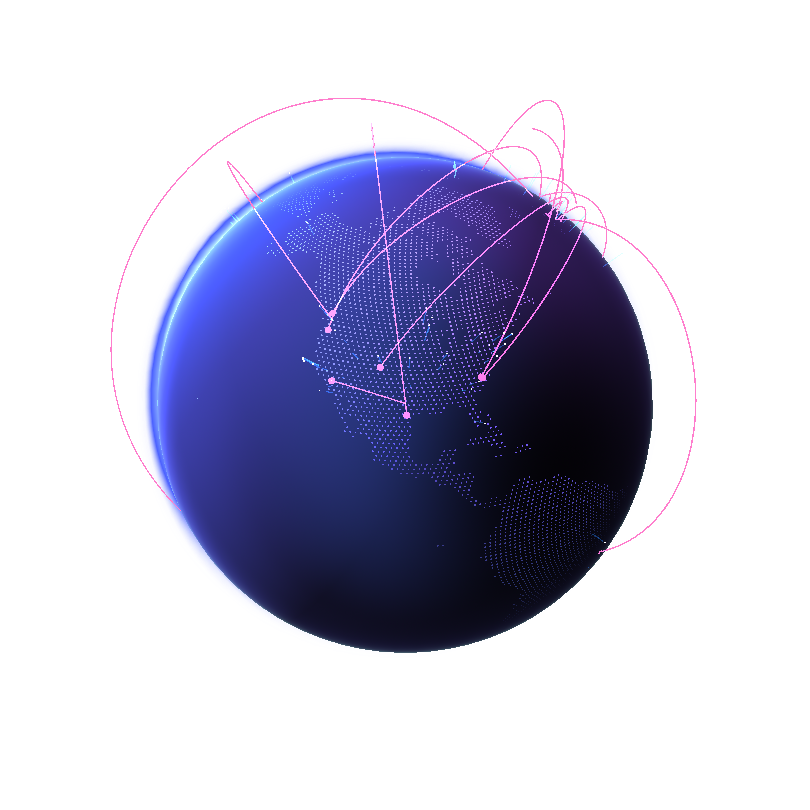
\includegraphics[width=0.7\linewidth]{images/screenshot001}
\caption{}
\label{fig:screenshot001}
\end{figure}
It contains a nicely deep blue coloured sphere, with an atmosphere, where the countries are stylized as dots, with lines representing messages being sent to and from the dots. It's a nice artistic touch, however I am more interested in their implementation, as analysing their process will greatly benefit my project. \\
Luckily, I encountered a blog post\footnote{https://github.blog/2020-12-21-how-we-built-the-github-globe/} which greatly describes their thought process and which algorithms they may have used to render this globe.
By reading through this blog post, I've learned a couple of things which I may use to integrate into my project:
\begin{itemize}
\item They used \verb|THREE.js| to render the globe.
\item They didn't use a texture mapped onto the sphere to represent the countries, instead they use about "12,000 five-sided circles to render the earths regions". In the blog post, they provided a small algorithm to create the regions.
\item They allowed the user to see their own location by marking a point on the globe. I think this is an interesting idea and I might do something similar in my project.
\item They drew the lines between regions using \textbf{Bezier Curves}:
\begin{lstlisting}
curve = CubicBezierCurve3(startLocation, ctrl1, ctrl2, endLocation)
\end{lstlisting}
\item They performance optimized their code. Since Github is massive, they probably need to do this so their globe runs smoothly on all machines. This may be an idea I need to focus on if my program becomes too slow, however since I am only rendering one sphere, I don't think this should be a problem. Should it be a problem, I may need to research ways of optimizing my code.
\end{itemize}

\newpage

\subsection{Earth Day 2018 - Plus 360 Degrees}
"Earth Day 2018 - Plus 360 Degrees"\footnote{https://earth.plus360degrees.com} is a cinematic experience over the earth. It was created for Earth Day to remind people about the beauty and uniqueness of the planet. \\
\begin{figure}[h]
\centering
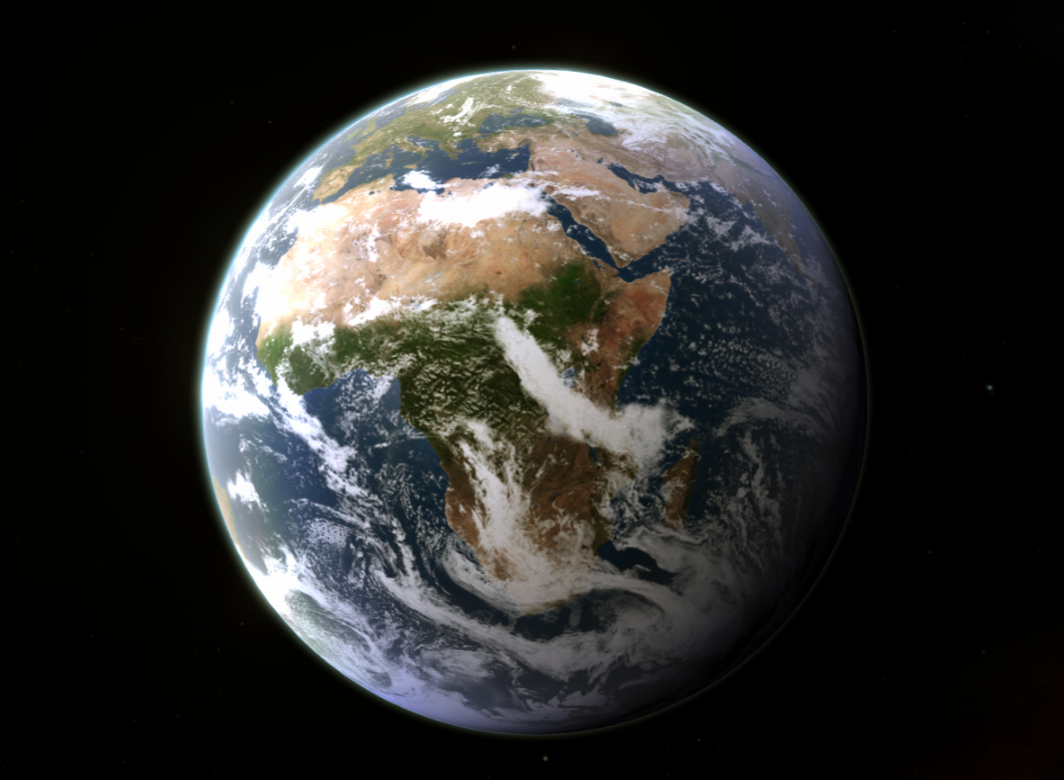
\includegraphics[width=0.7\linewidth]{images/screenshot002}
\caption{}
\label{fig:screenshot002}
\end{figure}

This website creates a beautiful and realistic representation of the earth. The fact that you can run this on your browser amazes me, so I think it would be smart to try and take some things down. Unfortunately, this isn't such a simple case as Github, there is very little information on how they created the website. However, in their credits\footnote{https://earth.plus360degrees.com/credits/} they do include some information.
\begin{itemize}
\item They rendered the earth with \verb|THREE.js|
\item They animated the sphere with \verb|Greensock|
\end{itemize}
Some things I want to note, that I have thought of when seeing this website:
\begin{itemize}
\item I like the way they used the clouds, it adds a layer of realness, and I may incorporate this into my project using shaders or by layering a sort of transparent texture on top of the sphere.
\item Their world texture is very highly detailed, and I think that also adds a layer of realness. I think I want to focus on making my earth as 'real' as possible, as that may keep my client interested on my project.
\end{itemize}

\newpage

\subsection{Experiments with Google - WebGL Globe}
Google has featured in their 'blog' "Experiments with Google" a WebGL globe\footnote{https://experiments.withgoogle.com/chrome/globe}: "The WebGL Globe is an open platform for geographic data visualization. We encourage you to copy the code, add your own data, and create your own." \\
\begin{figure}[h]
\centering
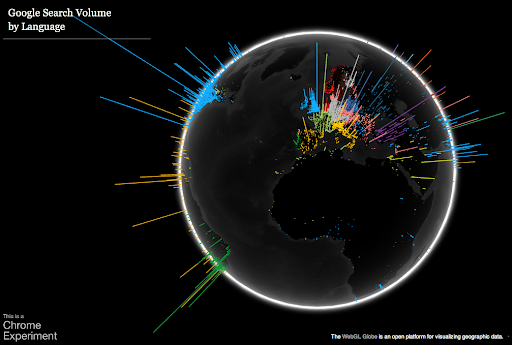
\includegraphics[width=0.7\linewidth]{images/screenshot003}
\caption{}
\label{fig:screenshot003}
\end{figure}

This is a project I may take a lot of inspiration from, as it features many of the features that I need in my project, and includes code\footnote{https://github.com/dataarts/webgl-globe} that I may take inspiration and learn from.
It features:
\begin{itemize}
\item Latitude / longitude data spikes
\item Color gradients based on data values
\item Mouse control and wheel to zoom
\end{itemize}
I analysed their code and development tactics, and picked out some things that I may use for my project.
\begin{itemize}
\item They render their sphere and data using \verb|THREE.js|
\item They format their data using \verb|JSON|
\item They render the data using boxes as 'points', here's some snippets of code that I found that show this, the comments start with '//' and are notes that I have taken:
\begin{lstlisting}
// Here they create the geometry for a point (as shown it is a box of a length)
geometry = new THREE.BoxGeometry(0.75, 0.75, 1);

// Each point is now a mesh of that box.
point = new THREE.Mesh(geometry);
\end{lstlisting}
That concludes my observation, however it doesn't show how they actually plot the points, that actually happens in a function \verb|createPoints()|:
\begin{lstlisting}
// This is how they determine the plot length
// _baseGeometry is a variable that contains data about where each point is, and each vertex of the point
var padding = 8-this._baseGeometry.morphTargets.length;
// Iterate through all points
for(var i=0; i<=padding; i++) {
	// Push all the vertices to the target where they will all be rendered
	this._baseGeometry.morphTargets.push({'name': 'morphPadding'+i, vertices: this._baseGeometry.vertices});
}
\end{lstlisting}
Furthermore, they have a function \verb|addPoint()|, which I find too verbose to feature here, however, I will take snippets of the function and analyse each one.
This is how they position each point, this will be extremely useful!
\begin{lstlisting}
// phi is the 'latitude'
// theta is the 'longitude'
// see https://en.wikipedia.org/wiki/Spherical_coordinate_system
var phi = (90 - lat) * Math.PI / 180;
var theta = (180 - lng) * Math.PI / 180;

// each point coordinate is positioned using a combination of trigonometric functions
// again, see https://en.wikipedia.org/wiki/Spherical_coordinate_system
point.position.x = 200 * Math.sin(phi) * Math.cos(theta);
point.position.y = 200 * Math.cos(phi);
point.position.z = 200 * Math.sin(phi) * Math.sin(theta);

// remember that point was declared before as a Mesh object, thus it is declared as an actual 3D object in the world.
\end{lstlisting}
\item They rendered the texture in the fragment shader, for which I will place a snippet of here. What I find interesting is that they render the texture on the shader, and not using \verb|THREE.js|, which provides a way of placing textures on a sphere. I analysed the Javascript code, and I noticed that their implementation of this is actually small. All it does is load the texture, and draws it using the fragment shader (all in two lines of code!). This gives me hope, perhaps the actual texturing job of the project may not be as difficult as I thought.
\begin{lstlisting}
uniform sampler2D texture;
varying vec3 vNormal;
varying vec2 vUv;
void main() {
  vec3 diffuse = texture2D( texture, vUv ).xyz;
  float intensity = 1.05 - dot( vNormal, vec3( 0.0, 0.0, 1.0 ) );
  vec3 atmosphere = vec3( 1.0, 1.0, 1.0 ) * pow( intensity, 3.0 );
  gl_FragColor = vec4( diffuse + atmosphere, 1.0 );
}
\end{lstlisting}
As can be noted, they sort of 'diffused' the world texture along with the atmosphere. My initial idea was to render a sphere, map a texture on the sphere and create another transparent sphere which acts as the atmosphere. This is not what Google decided to do, and instead combined the two into one sphere. I'm not sure what to take of this, and I just think that they are two different implementations of the same idea, and I don't think there is much benefit of doing it all in one sphere (I want to elevate the atmosphere a slight bit).
\item The user can 'drag' the sphere around with their mouse, this is definitely something I want to take notes in and integrate into my project.
\end{itemize}

\newpage

\section{Prospective Users and Client}
The goal of this section is to provide an insight as to my prospective users, with an example client. \\
The kind of prospective users I seek, are mainly students, potentially geologists or cartographers. My project allows them to rotate a virtual globe, and have a from-space view to the landmasses and oceans. Furthermore, they can click on countries, allowing them to read some useful data about the country. They can also try and test their knowledge of country borders, and try and guess which country they are clicking, to test their accuracy.

\subsection{Client}
My end user and client, Will, is a knowledge source for geography. He thought that my project idea was interesting, and that he would definitely enjoy testing his knowledge of country borders, and comparing the data of countries depending on their location and position of the globe. Me and Will discussed about some potential objectives for my project:
\begin{itemize}
    \item \textbf{Gamification} \\
        Will and I discussed about a way of gamifying my project, so as to make it more widely available for people who want to be entertained. He thought that creating a quiz would be interesting, for an addition to the user interface to contain the country name, and that the player had to find the country to win. \\
        In my opinion, this would definitely be a great addition to the project. However, I don't think that it is a very necessary addition.
\end{itemize}

\newpage

\section{Solution Proposals}
The goal of this section is to bring all that I have researched, and apply and transform these ideas onto my project. This research was essential and massively beneficial, and I have learned a lot of ideas. While researching, I was able to map these ideas onto my project in a high-level manner.

\subsection{Rendering of the globe}
This is crucial problem that I \textbf{had} to find a solution for. I needed to find an efficient, simple to implement method for rendering my globe. Thankfully, with the current and previous systems analysis, most of which use the same \verb|THREE.js| framework which I will be using, I think that I have a good overview of what I need to do.
Firstly, I must find an appropriate solution for the most basic and strapped down idea, which is actually displaying the sphere. After some research into \verb|THREE.js|, this is what I have noted. \\ \\

In \verb|THREE.js|, objects are declared in three steps.
\begin{enumerate}
\item Firstly, the geometry of the object must be initialized. The geometry of an object is essentially data about the shape of the object. Since I am creating a globe, I should obviously use a spherical geometry.

\item Secondly, the material of the object must be declared. The material of an object is exactly what it describes. It is quite an arbitrary term, however I have found it to be defined as what will be displayed on the \textit{surface} of the object. This is a crucial step, as I need to somehow map the world, the landmasses, and the oceans on the surface of the sphere. From previous projects, each one does this step differently. For example, one of them doesn't map the texture on the material, and instead uses a fragment shader to colour each pixel the same colour as the texture. One other project may use the \verb|THREE.js| '\verb|MeshBasicMaterial|' which already allows for texture mapping as a parameter. \\
I think, that for my project I should keep it simple and do it the second way, which is simply using the already present \verb|THREE.js| method. However, if I should have some time to spare and to improve the graphics of my project, I may switch to using a shader as it provides much more control.

\item Thirdly, and finally, the mesh of the object is declared. The mesh is the final step to the object and contains data about the position of the object, it's orientation, and other physical attributes. It combines the material and geometry of the object and can finally be displayed on the screen. This is a simple task in \verb|THREE.js| and can easily be done in a single line of code. Further on in the code, for example, if I need to rotate the sphere, I can use the mesh of the object's rotation property to rotate it.
\end{enumerate}

\subsection{User Input}
This is another crucial problem for which I must prepare for. User input is a crucial part of my project as it is how the user will interact with the project. For the most part, I don't think that I will require any keyboard input, as all of the functionality can be available with just the mouse; this is useful as I can just focus on mouse input, keeping my project simple.
Here are some proposals on how I may solve this problem:
\begin{itemize}
\item The sphere must rotate on some form of input. Previously, where I analysed some real examples of current systems, I noticed that most of them do this by using mouse dragging. When the mouse button is held and moved, the sphere rotates accordingly. This is the method of input I will be using for my project. The way I am thinking of approaching this problem, is by registering some sort of 'event' when the user holds down the mouse button. When the mouse button is held down, the sphere can rotate along with the mouse. I should experiment with the sensitivity of which the sphere rotates, so as to not make it too slow at rotating, or too fast.

\item When a country is clicked, an information pop up should appear. Keeping it in topic, I will focus on the mouse input for this bullet point. \\
The way I am thinking of approaching this, is by sending out some sort of an invisible 'ray' on a mouse click. When this 'ray' intersects a country, it should display the appropriate information about the country. This will be quite a complex problem, and will definitely require some experimentation and deep algorithms / maths further on.
\end{itemize}

\subsection{API requests \& country information}
This is another crucial problem for which I should pre-emptively solve. The basic overview of this problem is that I need to create a method of requesting the API, formatting the data, and displaying the formatted data on user input. I will split this problem into steps:
\begin{enumerate}
\item \textbf{API requests} \\
During previous research into APIs, I concluded that there were two main APIs that I will use to request and gather the information needed to be displayed. To put it in simple terms, I need to send a request to a server, which will in turn send my desired data back to be processed. This is quite a simple problem, and thus I don't think that it will require much thought, it is however quite important that I get this right.

\item \textbf{Formatting the data} \\
We need to format this data which is sent back to us in a manner where the user can read it, and that the developer can also easily manipulate and store the data. This problem is quite API specific, but from what I have researched and through example requests, I think I can simply retrieve the data, and simply store it in a Javascript object. Each country has its own slight differences in data, and so I will need to deal with this accordingly. This data must then be formatted in a way that the user can read it, so numbers should be displayed in a readable format.

\item \textbf{Displaying the data} \\
My thought towards displaying the data is to, on user input, create a dialogue box, near or next to the cursor. This can be done using \verb|THREE.js| 2D objects. Inside the dialogue box, the data must be presented in a readable fashion. Overall, the dialogue box should fit with the theme of the project, and so must the data. \\
The data could be presented in a multitude of ways, such as small graphs inside the dialogue box or text. This will be something I should think about later in the project, but however is not very high priority. Initially, I think that I will simply just render text inside the dialogue box.
\end{enumerate}

\subsection{Formatting}
This is an 'optional' step, once I have the data layed out from the API queries, I can work on formatting the data so the user can see the data. I want this to be as user friendly as possible, so that anyone can use the website, and understand the data being displayed. I have some ideas layed out for this:
\begin{itemize}
    \item \textbf{User Interface}
        I think a vertical bar on the right side of the screen, containing each bit of data, each item being layed out on top of another, would be a good final user interface I can work towards.
    \item \textbf{Graphs}
        This is an ambitious step, however having graphs would definitely be a plus, as the user can easily see how the data changes through time.
\end{itemize}

\subsection{Graphics}
Another 'optional' step, I can make the user input more user friendly and tactile if I add some sort of feedback to the globe.
\begin{itemize}
    \item A little idea I have, which stems from the Github globe, is how they have lines coming to and from countries. For example, when you click on the globe, a line can stem from the position clicked to the country selected.
    \item Another interesting idea which I have thought of, is having two world textures, one where the countries are in greyscale, and one where the countries are in color - wherever the mouse hovers, a diffusion occurs between the two textures and the greyscale emerges radially from the cursor.
    \item I think that stars would be a great addition to the project, and to also make each of them blink. Since I need thousands of stars, I need to think about how I can optimize the large amount of stars, so as to not slow down the webpage.
\end{itemize}
\newpage
\section{Modelling of Problem}
My project can be modelled in a series of connective flow diagrams:
\subsection{Rendering \& Animating}
\begin{figure}[h]
\centering
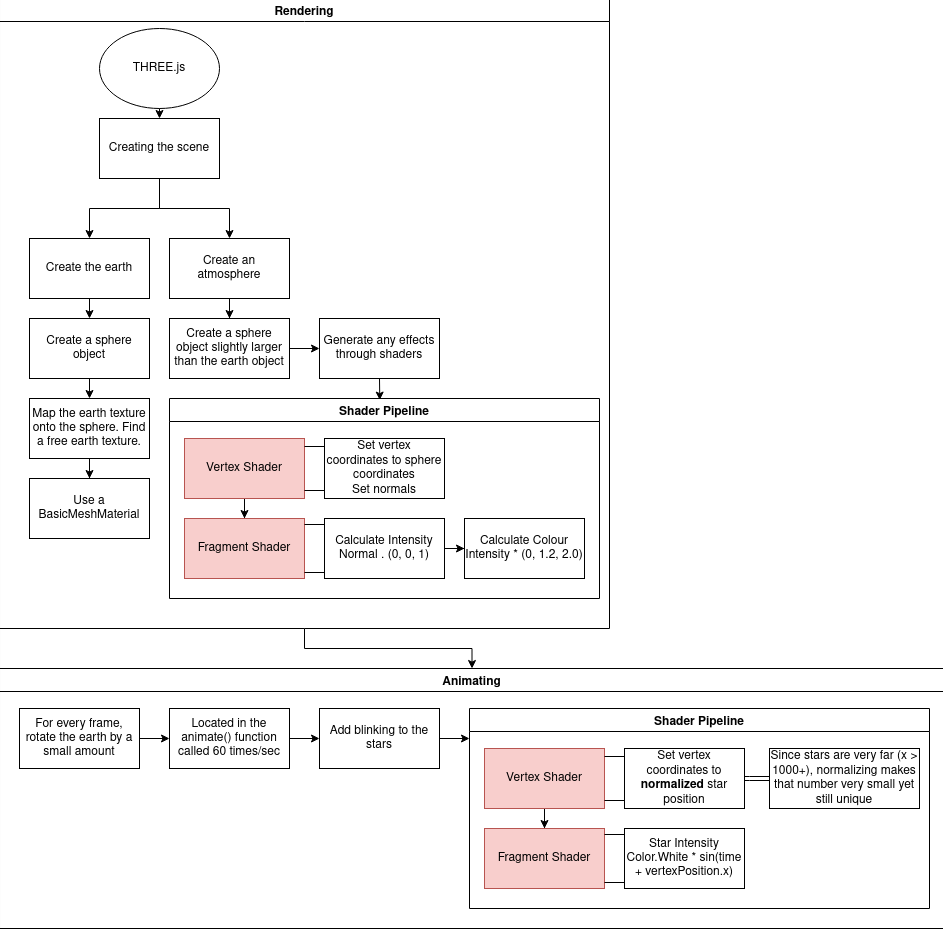
\includegraphics[width=1.0\linewidth]{images/renderanimate}
\caption{}
\label{fig:renderanimate}
\end{figure}

\newpage
\subsection{User Input}
\begin{figure}[h]
\centering
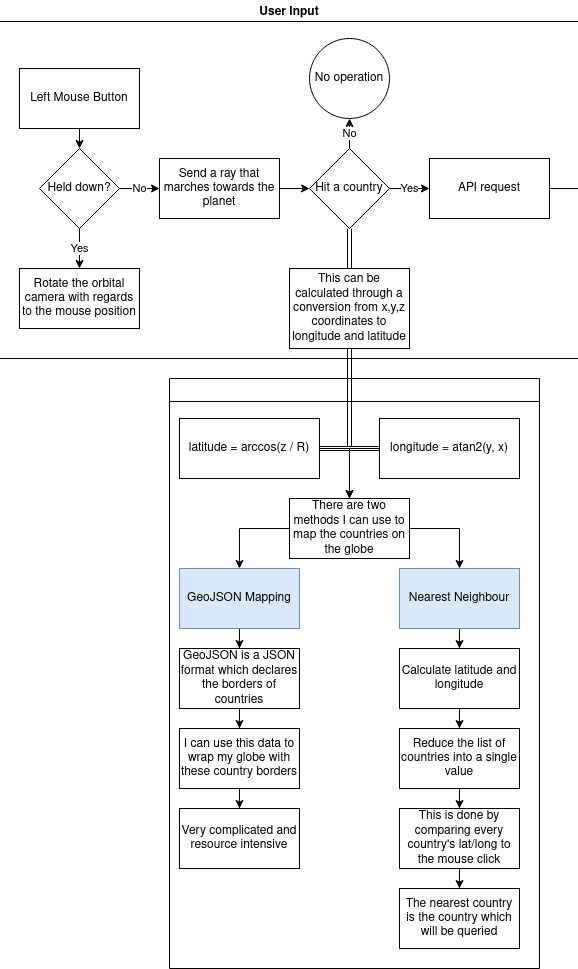
\includegraphics[width=0.6\linewidth]{images/input}
\caption{}
\label{fig:input}
\end{figure}

\newpage
\subsection{API Querying}
\begin{figure}[h]
\centering
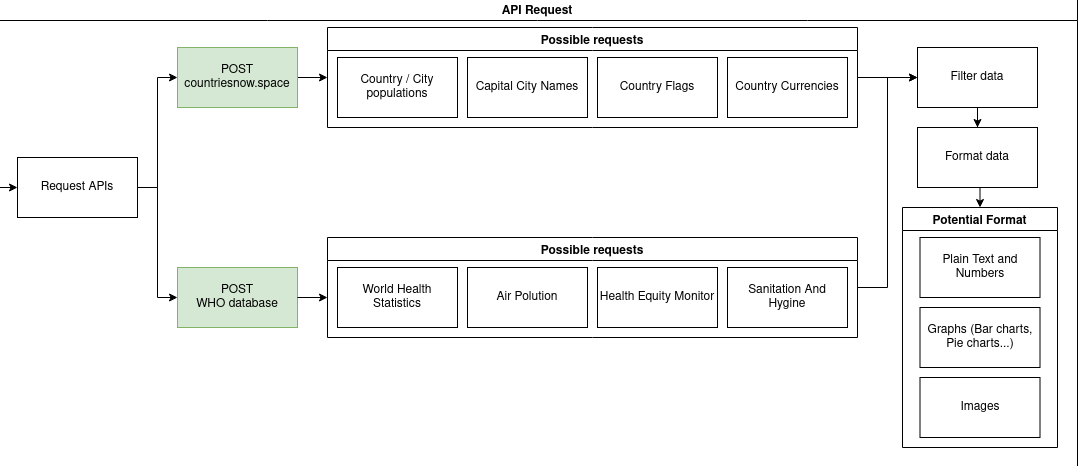
\includegraphics[width=1.0\linewidth]{images/apireq}
\caption{}
\label{fig:apireq}
\end{figure}

\subsection{Conclusionary Model}
\begin{figure}[h]
\centering
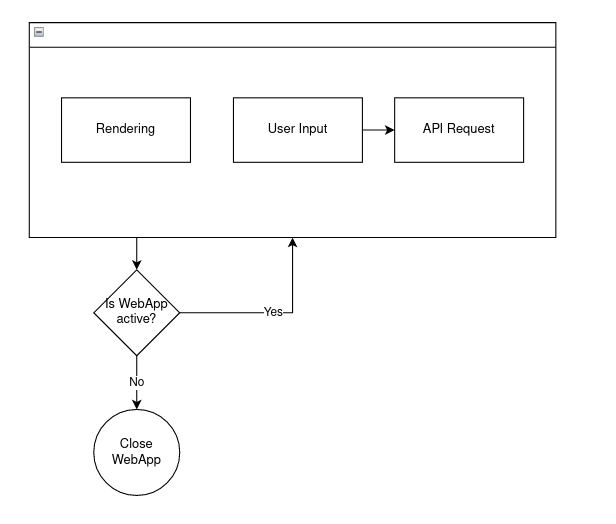
\includegraphics[width=0.63\linewidth]{images/conclusionary}
\caption{}
\label{fig:conclusionary}
\end{figure}


\newpage
\section{Critical Path of Stages}
Each objective can be ranked and sorted by importance:
\begin{itemize}
    \item \textbf{Rendering the Globe} \\
        This is the core of the web application, without the globe, the web application would be bare. Thus, this is the most important step, and the first step to be completed.
    \item \textbf{User Input} \\
        User input controls whether the user can rotate and see the entirety of the globe, and it also dictates which country is selected, which can then be sent off as requests to the suitable APIs. Therefore, this is the second most important objective that needs to be completed.
    \item \textbf{API Requesting} \\
        Ultimately, and also importantly, the selected country must be sent to one or many API servers to retrieve useful data. This is not so simple, as there are also other steps involved:
        \begin{itemize}
            \item \textbf{Formatting} \\
                The API response must be formatted so as to be readable to the user.
            \item \textbf{Displaying} \\
                The API response must then be displayed to the user. This section will be written in HTML and CSS.
        \end{itemize}
    \item Additional Objectives:
        \begin{itemize}
            \item \textbf{Graphical Improvement} \\
                Eye candy such as stars. Improvements to the API UI in general.
            \item \textbf{Optimization} \\
                Depending on how slow our webpage is, we may need to apply some layers of optimization to make our webpage faster, and more responsive.
        \end{itemize}
\end{itemize}

\newpage
\section{Objectives}
Through the research I have compiled, I can determine the main future objectives that I have to work towards.

\subsection{Main objectives}
\begin{itemize}
    \item \textbf{Rendering}
        I obviously need to render the globe, that is of upmost importance, the whole web application \textit{is} based on the globe after all.
    \item \textbf{User Input}
        The next main objective involves user input - I need the user to be able to move the globe around, and be able to select countries using the mouse.
    \item \textbf{API Querying}
        I need the user to be able - depending on the selection - to recieve information about the country. This involves API querying, JSON, text formatting and CSS \& HTML.
\end{itemize}

\subsection{Additional \& Further objectives}
When I overcome the challenges of the main objectives, I can then focus on working towards extra, optional objectives.
\begin{itemize}
    \item \textbf{Formatting}
        When I have a basic, simple UI which displays some information about the country which is selected, I can start displaying more data.
    \item \textbf{Graphics}
        I can also work on making the globe and the interactions have greater user feedback by using graphics. For example, a line which connects to the country to signal that you have clicked it. I think some stars would also make the project look more inviting.
    \item \textbf{Graphs}
        If time is available, I can work on converting simple number data, into graphical data with plots. Since the APIs provide a wide range of time for each data point, I can plot the data.
\end{itemize}

\newpage
\section{User Requirements}
A reason that I picked a webpage based approach to the entire project, was that webpages usually load the same for all computers. A problem which arises is old web browsers such as Internet Explorer, which do not support a lot of the recent Javascript and CSS versions. Since my project does not use complex CSS, I don't expect that to be a problem. However, I need to be aware of bugs that may appear on older web browsers, and test my webpage on a multitude of web browsers. \\
In conclusion, there is no user requirement, except for a \textbf{web browser}.
